% Generated by pysimcount.pfseeds -- do not edit; regenerate instead.
% figure: B-order6-by-formula -- Every order-6 formula at measured r; median over seeds [1, 2, 3, 4, 5, 6, 7, 8, 9, 10], bars = min..max
% metric=total gatebase=cz merged
% seed 1: git_commit=01d3c275ceae2840002bd1aaea68f59b987c4975 git_dirty=False
% seed 2: git_commit=01d3c275ceae2840002bd1aaea68f59b987c4975 git_dirty=False
% seed 3: git_commit=01d3c275ceae2840002bd1aaea68f59b987c4975 git_dirty=False
% seed 4: git_commit=01d3c275ceae2840002bd1aaea68f59b987c4975 git_dirty=False
% seed 5: git_commit=01d3c275ceae2840002bd1aaea68f59b987c4975 git_dirty=False
% seed 6: git_commit=01d3c275ceae2840002bd1aaea68f59b987c4975 git_dirty=False
% seed 7: git_commit=01d3c275ceae2840002bd1aaea68f59b987c4975 git_dirty=False
% seed 8: git_commit=01d3c275ceae2840002bd1aaea68f59b987c4975 git_dirty=False
% seed 9: git_commit=01d3c275ceae2840002bd1aaea68f59b987c4975 git_dirty=False
% seed 10: git_commit=01d3c275ceae2840002bd1aaea68f59b987c4975 git_dirty=False
% derived: B-order6-by-formula.tex restyled by pysimcount.figuniform: extrapolated points (r from power-law fit) drawn in their series' measured style, style-key legend entries removed; extrapolated n = [13, 20]; source_sha256=2ba70a8490c448d8653e448d0ad3c4ac4ff0134a33c5edfaf43e555ad0374ffd
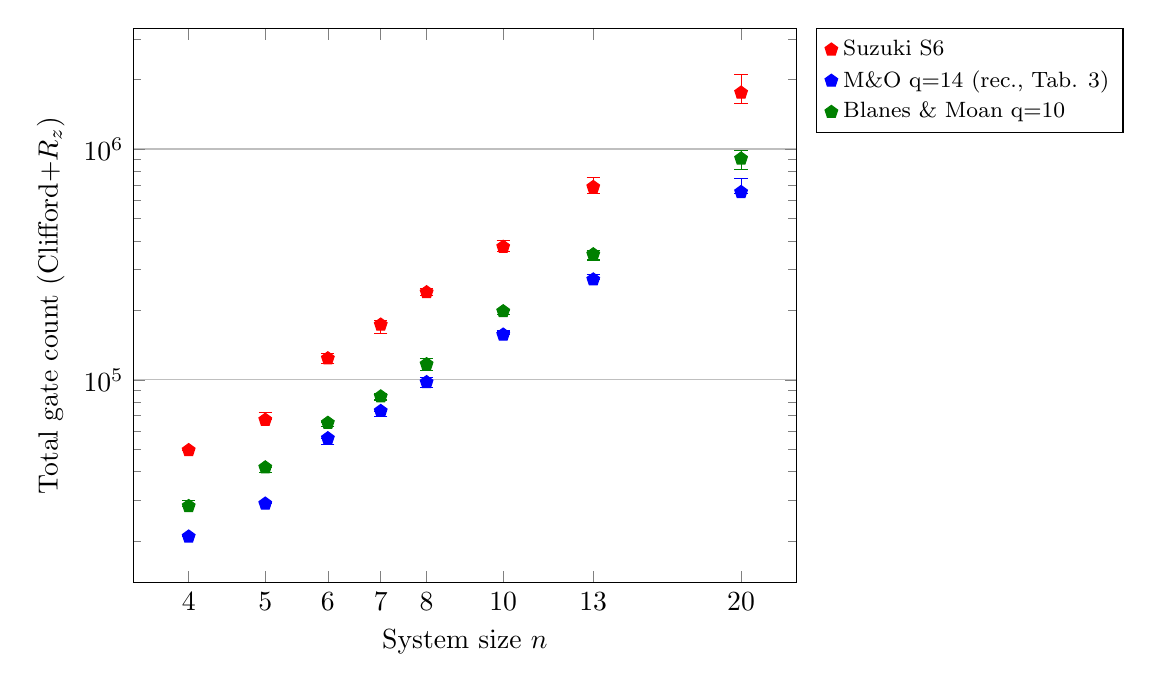
\begin{tikzpicture}
  \begin{loglogaxis}[
    width=10cm,
    xlabel={System size $n$},
    ylabel={Total gate count (Clifford+$R_z$)},
    xtick={4,5,6,7,8,10,13,20},
    xticklabels={4,5,6,7,8,10,13,20},
    ymajorgrids=true,
    legend pos=outer north east,
    legend cell align=left,
    legend style={font=\footnotesize},
  ]
    \addplot[only marks, red, mark=pentagon*, mark size=2.4pt, mark options={solid, fill=red}, error bars/.cd, y dir=both, y explicit, error bar style={red}] coordinates {
      (4,49536) += (0,0) -= (0,0)
      (5,67080) += (0,5160) -= (0,0)
      (6,123840) += (0,6192) -= (0,6192)
      (7,173376) += (0,7224) -= (0,14448)
      (8,239424) += (0,8256) -= (0,8256)
      (10,376680) += (0,25800) -= (0,15480)
    };
    \addlegendentry{Suzuki S6}
    \addplot[only marks, red, mark=pentagon*, mark size=2.4pt, mark options={solid, fill=red}, forget plot, error bars/.cd, y dir=both, y explicit, error bar style={red}] coordinates {
      (13,684216) += (0,67080) -= (0,40248)
      (20,1754400) += (0,350880) -= (0,185760)
    };
    \addplot[only marks, blue, mark=pentagon*, mark size=2.4pt, mark options={solid, fill=blue}, error bars/.cd, y dir=both, y explicit, error bar style={blue}] coordinates {
      (4,20916) += (0,0) -= (0,0)
      (5,29050) += (0,0) -= (0,0)
      (6,55776) += (0,0) -= (0,3486)
      (7,73206) += (0,0) -= (0,4067)
      (8,97608) += (0,4648) -= (0,4648)
      (10,156870) += (0,5810) -= (0,0)
    };
    \addlegendentry{M\&O q=14 (rec., Tab. 3)}
    \addplot[only marks, blue, mark=pentagon*, mark size=2.4pt, mark options={solid, fill=blue}, forget plot, error bars/.cd, y dir=both, y explicit, error bar style={blue}] coordinates {
      (13,271908) += (0,15106) -= (0,0)
      (20,650720) += (0,92960) -= (0,11620)
    };
    \addplot[only marks, green!50!black, mark=pentagon*, mark size=2.4pt, mark options={solid, fill=green!50!black}, error bars/.cd, y dir=both, y explicit, error bar style={green!50!black}] coordinates {
      (4,28356) += (0,1668) -= (0,0)
      (5,41700) += (0,0) -= (0,2085)
      (6,65052) += (0,0) -= (0,2502)
      (7,84651) += (0,2919) -= (0,2919)
      (8,116760) += (0,6672) -= (0,6672)
      (10,198075) += (0,2085) -= (0,6255)
    };
    \addlegendentry{Blanes \& Moan q=10}
    \addplot[only marks, green!50!black, mark=pentagon*, mark size=2.4pt, mark options={solid, fill=green!50!black}, forget plot, error bars/.cd, y dir=both, y explicit, error bar style={green!50!black}] coordinates {
      (13,349654) += (0,13552) -= (0,18974)
      (20,909060) += (0,75060) -= (0,91740)
    };
  \end{loglogaxis}
\end{tikzpicture}
